\documentclass[tikz,border=5pt]{standalone}
\usepackage{tikz}
\usetikzlibrary{arrows.meta, positioning, fit}

\begin{document}

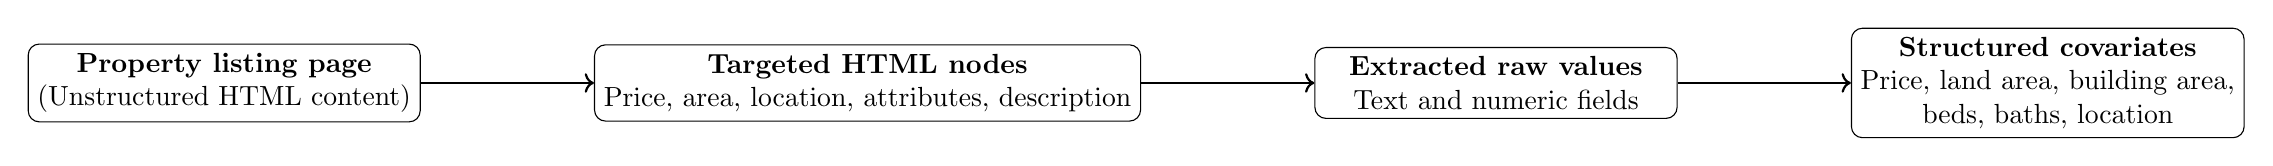
\begin{tikzpicture}[
  every node/.style={
    draw,
    rounded corners,
    align=center,
    minimum width=4.6cm,
    minimum height=9mm
  },
  arrow/.style={->, thick},
  node distance=10mm
]

% Raw page
\node (html) {
\textbf{Property listing page}\\
(Unstructured HTML content)
};

% Extracted elements
\node (nodes) [right=22mm of html] {
\textbf{Targeted HTML nodes}\\
Price, area, location, attributes, description
};

% Parsed values
\node (values) [right=22mm of nodes] {
\textbf{Extracted raw values}\\
Text and numeric fields
};

% Final dataset
\node (vars) [right=22mm of values] {
\textbf{Structured covariates}\\
Price, land area, building area,\\
beds, baths, location
};

% Arrows
\draw[arrow] (html) -- (nodes);
\draw[arrow] (nodes) -- (values);
\draw[arrow] (values) -- (vars);

\end{tikzpicture}

\end{document}
